% main.tex -- Article for Nature Communications: the GYNI causal inequality.
% Companion files: si.tex (Supplementary Information), refs.bib, figures/ (generated by figures/make_figures.py).
% All decimals are directed-rounded from the stored exact rationals: lower bounds DOWN, upper bounds UP.
\documentclass[11pt]{article}

\usepackage[a4paper,margin=2.5cm]{geometry}
\usepackage{amsmath,amssymb,amsthm}
\usepackage{bm}
\usepackage{graphicx}
\usepackage{booktabs}
\usepackage{setspace}
\usepackage{lineno}
\usepackage[super,sort&compress,comma]{natbib}
\usepackage[colorlinks=true,linkcolor=blue,citecolor=blue,urlcolor=blue]{hyperref}
\usepackage{authblk}
\usepackage[font=small,labelfont=bf]{caption}
\setlength{\textfloatsep}{12pt plus 2pt minus 2pt}

\newtheorem{theorem}{Theorem}
\newtheorem{lemma}{Lemma}

\newcommand{\Tr}{\operatorname{Tr}}
\newcommand{\ket}[1]{\lvert #1\rangle}
\newcommand{\bra}[1]{\langle #1\rvert}
\newcommand{\one}{\mathbb{I}}
\newcommand{\tp}{\mathsf{T}}
\newcommand{\CC}{\mathbb{C}}
\newcommand{\RR}{\mathbb{R}}
\newcommand{\ZZ}{\mathbb{Z}}
\newcommand{\Igy}{I_{\mathrm{GYNI}}}
\newcommand{\Imax}{I_{\mathrm{GYNI}}^{\max}}
\newcommand{\cW}{\mathcal{W}}

\title{Pinning down the maximal quantum violation of the guess-your-neighbour's-input causal inequality}
\author[1]{Ansh Mishra}
\author[2]{Aryan Senthilkumar}
\affil[1]{Independent researcher, Cumming, GA, USA}
\affil[2]{Independent researcher, Johns Creek, GA, USA}
\date{}

\begin{document}
\maketitle

\begin{abstract}
\noindent
Causal inequalities bound the correlations that parties acting in a definite causal order can produce, and the process-matrix framework, which keeps quantum theory in every local laboratory but drops a global causal order, violates them. The largest possible violations, the analogues of Tsirelson's bound for Bell inequalities, are known only in a few cases. For the guess-your-neighbour's-input (GYNI) inequality, one of the two simplest bipartite causal inequalities, the maximal success probability was known only to lie between 0.6219 and 0.7592. Here we prove that it lies between 0.622165901353 and 0.622183755532, an interval about 7,700 times narrower. The upper bound comes from a new dimension-free hierarchy of semidefinite relaxations for process-matrix correlations, certified at level eight by an exact rational dual certificate. The lower bound is an explicit process, verified in exact arithmetic. Both bounds, including the soundness of the hierarchy, are machine-checked in the Lean proof assistant.
\end{abstract}

\onehalfspacing
\linenumbers

\section*{Introduction}

In standard quantum theory the operations performed by different parties are embedded in a fixed causal structure: each party acts either before, after, or independently of the others. Whether this assumption can be relaxed has been studied in approaches to quantum gravity\cite{Hardy2007} and in quantum information, where superpositions of causal orders such as the quantum switch\cite{Chiribella2013} offer advantages in computation and communication\cite{Araujo2014,Guerin2016,Ebler2018} and have been realised in photonic experiments\cite{Procopio2015,Rubino2017}. Oreshkov, Costa and Brukner introduced process matrices to describe the most general correlations that local quantum laboratories can share when no global causal order is assumed\cite{Oreshkov2012}. Correlations compatible with a definite causal order, or with a probabilistic mixture of such orders, satisfy linear \emph{causal inequalities}\cite{Oreshkov2012,Branciard2016,OreshkovGiarmatzi2016,Abbott2016}, and process matrices can violate them\cite{Oreshkov2012}; see ref.~\citenum{Costa2026review} for a recent review. Processes such as the quantum switch produce only causal correlations, and whether processes that violate causal inequalities can be realised physically is a subtle question\cite{PurvesShort2021,Wechs2023}.

How strongly can causal inequalities be violated? For Bell inequalities the corresponding question is answered by Tsirelson bounds\cite{Tsirelson1980}, which the hierarchy of semidefinite programs (SDPs) of Navascu\'es, Pironio and Ac\'in computes systematically\cite{NPA2007,NPA2008,Brunner2014}. For causal inequalities, rigorous upper bounds on process-matrix violations are much more recent\cite{Brukner2015,LiuChiribella2025}. Liu and Chiribella derived an SDP bound for every causal inequality and determined the exact maximal violations for a class of inequalities that includes the ``lazy'' guess-your-neighbour's-input (LGYNI) inequality and a biased version of the original inequality of ref.~\citenum{Oreshkov2012}; they suggested that their relaxation may be the first level of a hierarchy\cite{LiuChiribella2025}.

The guess-your-neighbour's-input (GYNI) inequality and LGYNI represent the two families of nonequivalent causal inequalities in the simplest bipartite scenario, with binary inputs and outputs\cite{Branciard2016}. For GYNI the gap between the known bounds remained large. The best upper bound valid in all dimensions was $0.7592$ (ref.~\citenum{LiuChiribella2025}), whereas see-saw optimisation in fixed dimensions found $0.6218$ in local dimension five\cite{Branciard2016} and $0.6219$ in dimensions six and seven\cite{BoghiuSimonov2026}. The maximal violation was stated as open in these works and in the recent review\cite{Branciard2016,LiuChiribella2025,BoghiuSimonov2026,Costa2026review}.

Here we determine it to within $1.79\times10^{-5}$. We introduce a hierarchy of SDP relaxations for process-matrix correlations, prove that every level is a valid dimension-independent upper bound, and certify level eight with an exact rational certificate. We also construct an explicit strategy that nearly attains the bound. All steps are checked in exact arithmetic, and both bounds, including the soundness of the hierarchy, are formally verified in the Lean~4 proof assistant\cite{Lean4} with the Mathlib library\cite{Mathlib2020}.

\section*{Results}

\subsection*{The GYNI game}
Alice has input and output spaces $A_I,A_O$ and Bob has $B_I,B_O$, all of finite dimension (Fig.~\ref{fig:game}). An instrument $\{M_{a|x}\}_a$ is a family of completely positive (CP) maps from operators on $A_I$ to operators on $A_O$ whose sum is trace preserving (TP); likewise $\{N_{b|y}\}_b$ for Bob. Using Choi operators $C_F=\sum_{ij}\ket{i}\bra{j}\otimes F(\ket{i}\bra{j})$ (ref.~\citenum{Choi1975}), a \emph{process} is an operator $W\succeq0$ on $A_I\otimes A_O\otimes B_I\otimes B_O$ with $\Tr[W(C_A\otimes C_B)]=1$ for all Choi operators $C_A,C_B$ of CPTP maps\cite{Oreshkov2012,Araujo2015}. A strategy $S=(W;M;N)$ produces the correlations $p(a,b|x,y)=\Tr[W(C_{M_{a|x}}\otimes C_{N_{b|y}})]$. Local ancillas and shared entanglement are included, as they can be absorbed into $W$.

\begin{figure}[t]
\centering
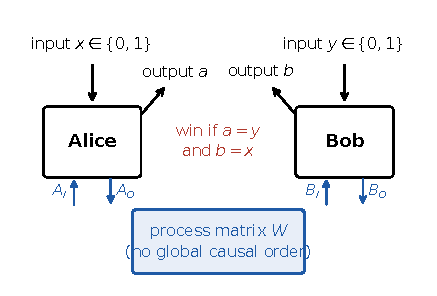
\includegraphics[width=0.55\textwidth]{figures/fig1_gyni_game.pdf}
\caption{\textbf{The GYNI game with a process matrix.} Alice and Bob receive uniformly random input bits $x$ and $y$ and output bits $a$ and $b$. Their laboratories receive quantum systems on the input spaces $A_I,B_I$ and send them out on $A_O,B_O$, connected by a process matrix $W$ that need not respect any global causal order. They win if $a=y$ and $b=x$. Causally ordered strategies win with probability at most $1/2$.}
\label{fig:game}
\end{figure}

In the GYNI game the parties receive independent uniformly random bits $x,y$ and output bits $a,b$; they win if each guesses the other's input. The success probability
\begin{equation}
\Igy=\frac14\sum_{x,y\in\{0,1\}}p(a=y,\,b=x\,|\,x,y)
\label{eq:gyni}
\end{equation}
is at most $1/2$ for every causal correlation\cite{Branciard2016}: in a definite causal order, at least one of the parties cannot be influenced by the other's input. We write $\Imax=\sup_S\Igy(S)$ for the supremum over strategies whose local systems have finite, but arbitrary, dimension.

\subsection*{Main result}

\begin{theorem}\label{thm:main}
$0.622165901353\;\le\;\Imax\;\le\;0.622183755532$.
\end{theorem}

The interval has width $1.79\times10^{-5}$, compared with $0.137$ before (Fig.~\ref{fig:bounds}). The upper bound is the certified value of the eighth level of the hierarchy introduced below, and the lower bound is the exact value of an explicit strategy. The two ingredients are independent of each other. Both are verified by stand-alone programs in integer or rational arithmetic, without any numerical solver\cite{repo}, and both are machine-checked in Lean (Fig.~\ref{fig:verification}).

\begin{figure}[t]
\centering
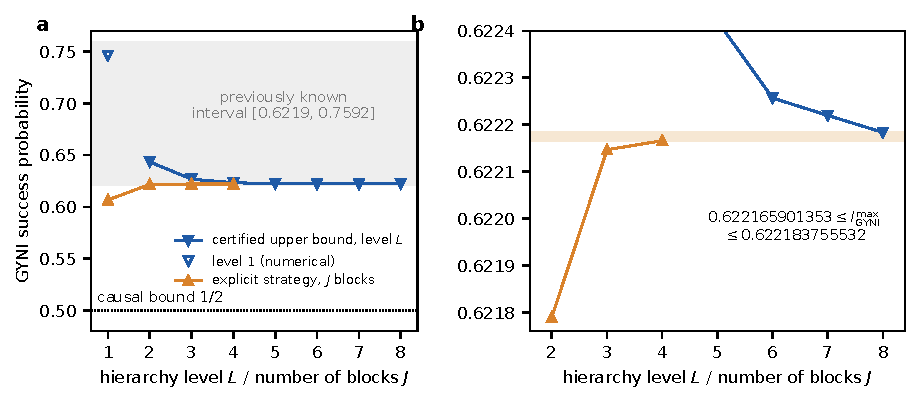
\includegraphics[width=\textwidth]{figures/fig2_bounds.pdf}
\caption{\textbf{Certified bounds on the maximal GYNI violation.} \textbf{a}, Certified upper bounds from levels $L=2,\dots,8$ of the hierarchy (blue, downward triangles; level one numerical, open symbol) and exact values of the explicit strategies with $J=1,\dots,4$ Jordan blocks (orange, upward triangles; $J=1$ numerical). The grey band is the previously known interval $[0.6219,0.7592]$. \textbf{b}, Close-up: the final interval $0.622165901353\le\Imax\le0.622183755532$ (shaded).}
\label{fig:bounds}
\end{figure}

\begin{figure}[t]
\centering
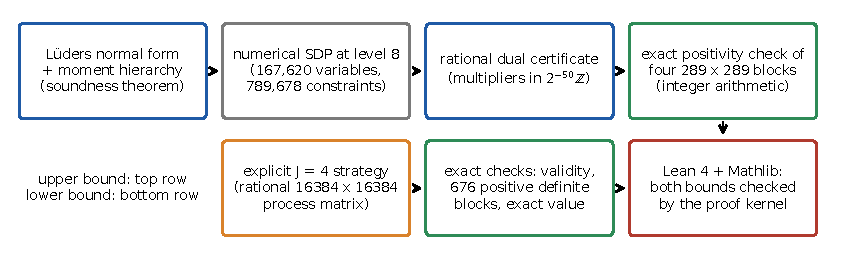
\includegraphics[width=\textwidth]{figures/fig3_verification.pdf}
\caption{\textbf{How the two bounds are established.} Top row: the upper bound follows from the L\"uders normal form and the soundness of the hierarchy, a numerical solution of the level-eight relaxation, its conversion to an exact rational dual certificate, and an exact positivity check in integer arithmetic. Bottom row: the lower bound is an explicit rational process checked in exact arithmetic. Both chains, including the soundness theorem, are verified by the Lean proof kernel.}
\label{fig:verification}
\end{figure}

\subsection*{A L\"uders normal form for local instruments}
The first step removes the generality of the instruments.

\begin{lemma}[L\"uders normal form]\label{lem:lueders}
For every strategy there are finite-dimensional spaces $H_A,H_B$, projective measurements $\{P_{a|x}\}_a$ on $H_A$ and $\{Q_{b|y}\}_b$ on $H_B$, and a process $\widetilde W$ with inputs $H_A,H_B$ and outputs $H_A\otimes X$, $H_B\otimes Y$ ($X=Y=\CC^2$), which reproduces $p(a,b|x,y)$ with the L\"uders instruments
\begin{equation}
\widetilde M_{a|x}(\rho)=P_{a|x}\rho P_{a|x}\otimes\ket{x}\bra{x}_X ,\qquad
\widetilde N_{b|y}(\sigma)=Q_{b|y}\sigma Q_{b|y}\otimes\ket{y}\bra{y}_Y .
\label{eq:lueders}
\end{equation}
Moreover, $\widetilde W$ is block diagonal in the register values.
\end{lemma}

Each instrument is dilated into a projective measurement on a larger space followed by a post-processing that depends on the setting; the setting-independent parts of the dilation and the setting-controlled post-processing are then absorbed into the process (Methods). In L\"uders form the two measurements of each party are described by two unitary involutions $O_x=P_{0|x}-P_{1|x}$.

\subsection*{A dimension-free moment hierarchy}
By the universal property of the free product, $g_x\mapsto O_x$ defines a unitary representation $\pi_A$ of the infinite dihedral group $G=\ZZ_2*\ZZ_2=\langle g_0,g_1\,|\,g_0^2=g_1^2=e\rangle$, whose elements are the reduced words $w=(x_1,\dots,x_n)$ with $x_i\neq x_{i+1}$. Let $\cW_L$ be the $2L+1$ words of length at most $L$. For $k=(w,r)\in\cW_L\times\{0,1\}$ we define the word vector $\ket{k}=(\one\otimes\pi_A(w))\ket{\Phi}\otimes\ket{r}$, with $\ket{\Phi}=\sum_i\ket{i}\ket{i}$, and analogously $\ket{l}$ for $l=(v,s)$ on Bob's side. The level-$L$ moment matrix is the Gram matrix of $\widetilde W$ on these vectors,
\begin{equation}
\Gamma[(k,l),(k',l')]=\bra{k,l}\widetilde W\ket{k',l'} .
\label{eq:gamma}
\end{equation}
Every probability $p(a,b|x,y)$, and hence $\Igy$, is a linear function $o(\Gamma)$ of this matrix, because $P_{a|x}=[\one+(-1)^aO_x]/2$.

The operator $\ket{k'}\bra{k}$ is the Choi operator of the map $\rho\mapsto\pi_A(w')\rho\,\pi_A(w)^\dagger\otimes\ket{r'}\bra{r}$, whose output partial trace is $\delta_{rr'}[\pi_A(w^{-1}w')]^\tp$. A combination of such operators therefore has a partial trace proportional to the identity \emph{in every realisation} whenever the corresponding identity holds in the group algebra $\RR[G]$. Validity of the process then enters through a factorisation lemma (Methods): the expectation of a product of two such combinations equals the product of their scalar traces. The certified relaxation of level $L$ consists of the following constraints on a real symmetric matrix $\Gamma$:
(V1) positivity, $\Gamma\succeq0$, which by Lemma~\ref{lem:lueders} amounts to four positive semidefinite blocks of size $n_L=(2L+1)^2$;
(V2) the linear constraints expressing validity of the process at the level of words;
(S) invariance under the symmetries of the game.

\begin{theorem}[Soundness]\label{thm:sound}
For every $L\ge1$ and every strategy $S$ with finite-dimensional local systems there is a real matrix $\Gamma$ satisfying (V1), (V2) and (S) with $o(\Gamma)=\Igy(S)$. Hence $\Imax\le\beta_L:=\sup\{o(\Gamma):\text{(V1), (V2), (S)}\}$.
\end{theorem}

Only the relations $g_x^2=e$ are used, never a relation specific to particular projectors, so the constraints hold in every dimension. The constraints of level $L$ are contained in those of level $L+1$, so $\beta_L$ does not increase with $L$. Positivity (V1) is the key new ingredient: level one already gives $\beta_1\approx0.7463$, below the bound $0.7592$ of ref.~\citenum{LiuChiribella2025}, which is reproduced at level two if (V1) is dropped and validity of the canonical processes of ref.~\citenum{LiuChiribella2025} is imposed instead. As consistency checks, the same hierarchy reproduces numerically, to solver precision, the exact LGYNI value $0.8194$ of ref.~\citenum{LiuChiribella2025} at level two and the value $(2+\sqrt2)/4$ for the game of ref.~\citenum{Oreshkov2012}.

\subsection*{A certified upper bound}
We solve the relaxations numerically and then certify each value with an exact dual certificate (Table~\ref{tab:levels} and Methods). Weak duality turns rational Lagrange multipliers $\lambda$ for the linear constraints into an upper bound $\lambda\cdot b$, provided that four matrices $Y_k(\lambda)$, defined exactly by stationarity, are positive semidefinite. We shift a numerical dual solution to make it strictly feasible, round its multipliers to rationals with denominator $2^{50}$, and check positive definiteness of the resulting integer matrices exactly, with all leading principal minors computed by fraction-free Bareiss elimination\cite{Bareiss1968}. Rounding numerical solutions to exact certificates in this way is standard in sum-of-squares optimisation\cite{PeyrlParrilo2008}.

At level eight the certified program has $167{,}620$ variables, $789{,}678$ linear constraints and four blocks of size $289$. The certificate gives
\begin{equation}
\beta_8\le\frac{175129158097837}{2^{48}}=0.6221837555310\ldots ,
\end{equation}
which proves the upper bound in Theorem~\ref{thm:main}. The margin used to make the certificate strictly feasible costs only $2.89\times10^{-7}$. A stand-alone verifier rebuilds all constraints, recomputes the four matrices from the stored integers and checks all minors in about eight minutes on one processor core. Independently of the proof, all $789{,}678$ constraints were evaluated on the moment matrices of more than $100$ strategies (general instruments passed through a separately written implementation of Lemma~\ref{lem:lueders}, generic L\"uders-form processes, see-saw optima, and the strategies below), with no residual above $2.1\times10^{-14}$ (Supplementary Note~6).

\begin{table}[t]
\centering
\caption{\textbf{Certified upper bounds on the level-$L$ value $\beta_L$, and hence on $\Imax$ (rounded up).} $n_L=(2L+1)^2$ is the size of each of the four positive semidefinite blocks and $m_L$ the number of linear constraints. The last column is the optimum returned by the interior-point solver (numerical, not rigorous); the certified bounds exceed it essentially by the margin $\varepsilon n_L$, with $\varepsilon=10^{-6}$ at $L=4$, $10^{-7}$ at $L=5,6,7$ and $10^{-9}$ at $L=8$. Entries marked $\dagger$ were certified in an equivalent formulation with words in the two projectors $P_{0|x}$ (Supplementary Note~4).}
\label{tab:levels}
\begin{tabular}{rrrll}
\toprule
$L$ & $n_L$ & $m_L$ & certified bound & numerical\\
\midrule
1 & 9   & --                    & --                          & 0.7462629\\
2 & 25  & $5{,}486^\dagger$     & $0.6434871^\dagger$         & 0.6434843\\
3 & 49  & $21{,}708^\dagger$    & $0.6267932^\dagger$         & 0.6267499\\
4 & 81  & $59{,}326$            & $0.6233558$                 & 0.6232747\\
5 & 121 & $134{,}604$           & $0.6224213$                 & 0.6224092\\
6 & 169 & $265{,}742$           & $0.6222569$                 & 0.6222399\\
7 & 225 & $475{,}300$           & $0.6222199$                 & 0.6221974\\
8 & 289 & $789{,}678$           & $\mathbf{0.622183755532}$   & 0.6221835\\
\bottomrule
\end{tabular}
\end{table}

\subsection*{An explicit strategy from coherently superposed Jordan blocks}
By Jordan's lemma\cite{Pironio2009}, two binary projective measurements decompose the local space into invariant blocks of dimension at most two, each characterised by one angle. This suggests the following family of L\"uders-form strategies, identical for Alice and Bob: $H=\CC^2\otimes\CC^J$ (a ``Jordan qubit'' and a label), the instruments of equation~\eqref{eq:lueders}, and
\begin{equation}
P_{0|x}=\sum_{j=1}^J\ket{\phi_j^x}\bra{\phi_j^x}\otimes\ket{j}\bra{j},\qquad
\ket{\phi_j^x}=\cos\tfrac{t_j}{2}\ket{0}+(-1)^{x+1}\sin\tfrac{t_j}{2}\ket{1},
\label{eq:jordan}
\end{equation}
so that the two measurement vectors in block $j$ enclose the angle $t_j$ (Fig.~\ref{fig:strategy}). For fixed angles the best process is the solution of an SDP, which we reduce with symmetries; the angles are optimised with gradients obtained from the envelope theorem (Methods).

\begin{figure}[t]
\centering
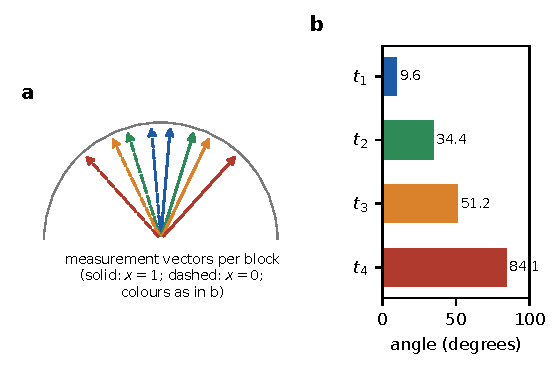
\includegraphics[width=0.6\textwidth]{figures/fig4_strategy.pdf}
\caption{\textbf{The explicit $J=4$ strategy.} \textbf{a}, In each Jordan block $j$ the two measurement vectors $\ket{\phi^0_j}$ (dashed) and $\ket{\phi^1_j}$ (solid) of equation~\eqref{eq:jordan} enclose the angle $t_j$; Alice and Bob use the same measurements. \textbf{b}, The four angles, $(9.6^\circ,34.4^\circ,51.2^\circ,84.1^\circ)$ rounded to $0.1^\circ$. The process is coherent across the blocks; a single block reaches only $0.6067$.}
\label{fig:strategy}
\end{figure}

A single block ($J=1$) reaches only $0.6067$. The higher values in Table~\ref{tab:strategies} come from processes that are \emph{coherent across blocks} with different angles: the label is not a classical flag but carries coherence that the process exploits. For $J=4$ the angles are $(t_1,\dots,t_4)=(9.59850^\circ,34.42477^\circ,51.18469^\circ,84.13806^\circ)$, chosen with rational $\tan(t_j/4)$ so that all entries of the measurements are rational. The process is a real $16384\times16384$ matrix with rational entries. A stand-alone verifier checks in exact arithmetic that it is a valid process, that it is block diagonal with $676$ blocks that are all positive definite, that the instruments are valid, and that
\begin{equation}
\Igy=0.62216590135390844\ldots ,
\end{equation}
a rational number with a $548$-bit denominator. This proves the lower bound in Theorem~\ref{thm:main}. The check uses no symmetry assumption and is independent of the hierarchy.

\begin{table}[t]
\centering
\caption{\textbf{Explicit $J$-block strategies of equation~\eqref{eq:jordan}}, with $d_{A_I}=2J$ and $d_{A_O}=4J$ (including the setting register); angles rounded to $0.1^\circ$, values rounded down. v: exact value, with all checks of the stand-alone verifier passed without symmetry assumptions. e: exact value, obtained with an earlier, symmetry-reduced positivity check (Supplementary Note~5). n: numerical optimum.}
\label{tab:strategies}
\begin{tabular}{cll}
\toprule
$J$ & angles $t_j$ (degrees) & $\Igy$\\
\midrule
1 & 36.1                   & $0.6067^{\rm n}$\\
2 & 22.7, 70.3             & $0.621789802^{\rm e}$\\
3 & 13.8, 40.2, 82.7       & $0.622146712690^{\rm v}$\\
4 & 9.6, 34.4, 51.2, 84.1  & $\mathbf{0.622165901353}^{\rm v}$\\
\bottomrule
\end{tabular}
\end{table}

\subsection*{Machine-checked proofs}
Both bounds of Theorem~\ref{thm:main} are formalised in Lean~4 with Mathlib, for every strategy with finite-dimensional local systems and with the standard definitions of processes and instruments. The theorem \texttt{gyni\_lower\_bound\_exact} exhibits the explicit process and instruments, proves that they are valid, and proves that their GYNI value equals the rational number above; positive semidefiniteness is established by kernel-checked integer certificates together with a proved party-swap symmetry. The theorem \texttt{gyni\_upper\_bound} states $\Igy\le175129158097837/2^{48}$ for every strategy. Its proof formalises the whole argument: Lemma~\ref{lem:lueders} (with an explicit Stinespring dilation and unitary completion), the factorisation lemma, the constraints (V1) and (V2), weak duality and the level-eight certificate, whose positivity is checked by the Lean kernel. Before the formal check the dual certificate is averaged over the symmetry group of the game; the averaged certificate is valid for the relaxation without (S), with the same bound, so the symmetry reduction is not needed in the formal proof. All theorems depend only on Lean's standard axioms. To our knowledge these are the first machine-checked bounds on the maximal violation of a causal inequality.

\section*{Discussion}

Theorem~\ref{thm:main} determines the maximal process-matrix violation of the GYNI inequality to within $1.79\times10^{-5}$, narrowing the previously known interval by a factor of about $7{,}700$. Nearly all of the remaining width is the gap of $1.76\times10^{-5}$ between the numerical level-eight optimum, $0.6221835$, and our lower bound; the margin of the certificate accounts for only $2.89\times10^{-7}$. A narrower interval therefore requires higher levels of the hierarchy or more Jordan blocks. Whether $\beta_L$ converges to $\Imax$ is open: unlike for the NPA hierarchy\cite{NPA2008} we have no convergence theorem, and the moment matrices we computed are not flat, so no optimal strategy can be read off from them. A geometric extrapolation of the numerical values in Table~\ref{tab:levels} gives about $0.62218$, but such extrapolations are heuristic and we make no claim about the exact value.

The explicit strategies show that the optimum requires coherence between Jordan blocks of different angles. A single block, the natural analogue of the qubit strategies that saturate Tsirelson's bound for the CHSH inequality, falls short by $0.0155$. The optimal violation is therefore not reached with a single qubit per party and a classical label, and the steady increase of the value with $J$ suggests that the supremum may only be approached as the number of blocks grows.

The method is not specific to GYNI. Lemma~\ref{lem:lueders} and the factorisation lemma do not refer to the game, and our implementation handles any number of settings with binary outcomes. We expect that the L\"uders normal form, applied party by party, together with a multilinear version of the factorisation lemma, extends the hierarchy to multipartite causal inequalities\cite{BaumelerWolf2014,Abbott2016}, where the structure of valid processes is richer\cite{Araujo2015,OreshkovGiarmatzi2016}; comparing with block-matrix relaxations\cite{DAlessandro2026} is a natural next step. Our bounds concern processes of finite dimension; the L\"uders normal form does not cover infinite-dimensional processes.

Finally, the combination of exact certificates with formal verification gives bounds that do not rely on the correctness of numerical solvers or of our own code: the Lean kernel checks the entire chain from the definition of a process to the final rational number. Formal verification has settled long-standing questions in mathematics\cite{Hales2017}; our results indicate that it can also deliver fully trustworthy bounds in quantum foundations, where Tsirelson-type bounds are increasingly obtained by large computer-assisted calculations.

\section*{Methods}

\subsection*{Processes, instruments and conventions}
We use the Choi operator $C_F=\sum_{ij}\ket{i}\bra{j}\otimes F(\ket{i}\bra{j})$. A process is an operator $W\succeq0$ with $\Tr[W(C_A\otimes C_B)]=1$ for all Choi operators $C_A,C_B$ of CPTP maps; equivalently, $W\succeq0$, $\Tr W=d_{A_O}d_{B_O}$ and $W$ lies in the subspace of valid processes\cite{Araujo2015}. Our Choi convention differs from that of ref.~\citenum{Oreshkov2012} by the transposition $W\mapsto W^\tp$, which maps processes onto processes and leaves $\Imax$ unchanged. Complete definitions are in Supplementary Note~2.

\subsection*{Proof of the L\"uders normal form}
Each instrument is written as $M_{a|x}(\rho)=\sum_eT_{x,e}P_{a|x}J\rho J^\dagger P_{a|x}T_{x,e}^\dagger$, with a fixed isometry $J$ from $A_I$ into $H_A$, projectors $P_{a|x}$ obtained from a unitary completion of the Stinespring isometry of $\{M_{a|x}\}_a$, and Kraus operators $T_{x,e}$ of a channel. The setting-independent pre-processing $J$ and the post-processing, which is controlled by the setting register, are absorbed into $\widetilde W=(\Phi_A^\dagger\otimes\Phi_B^\dagger)(W)$, where $\Phi_A(C)=\sum_{x,e}\hat K_{x,e}C\hat K_{x,e}^\dagger$ with $\hat K_{x,e}=J^\tp\otimes T_{x,e}\otimes\bra{x}_X$ maps Choi operators of channels to Choi operators of channels. The transpose is essential: pre-composition with $J$ acts on Choi operators as $C\mapsto(J^\tp\otimes\one)C(J^\tp\otimes\one)^\dagger$, whereas $J^\dagger$ in place of $J^\tp$ would implement pre-composition with the complex-conjugate isometry, which for complex $J$ does not reproduce the statistics. The full proof is in Supplementary Note~3.

\subsection*{Factorisation lemma}
Let $W$ be a process and let $C_A$, $C_B$ be arbitrary, not necessarily Hermitian, operators with $\Tr_{A_O}C_A=\lambda_A\one$ and $\Tr_{B_O}C_B=\lambda_B\one$. Then $\Tr[W(C_A\otimes C_B)]=\lambda_A\lambda_B$. Indeed, every such $C_A$ is a complex linear combination $\sum_i\alpha_iC_i$ of Choi operators of CPTP maps with $\sum_i\alpha_i=\lambda_A$ (Supplementary Note~3), and the claim follows by bilinearity.

\subsection*{The relaxation}
With $\langle c\otimes d,\Gamma\rangle:=\sum c_{kk'}d_{ll'}\Gamma[(k,l),(k',l')]$, constraint (V2) reads $\langle c\otimes d,\Gamma\rangle=\lambda_A\lambda_B$ whenever $c$ and $d$ have scalar traces $\lambda_A$ and $\lambda_B$ in the group algebra. These constraints are spanned by differences of pairs with the same group element $w^{-1}w'$ (``trace annihilating'') combined with such differences or with the pair of empty words (``trace preserving'') on the other side. The symmetries (S) are party exchange and the relabellings $(x\to1-x,\,b\to1-b)$ and $(y\to1-y,\,a\to1-a)$; in the dihedral word basis they act by signed permutations. The proof of Theorem~\ref{thm:sound} combines Lemma~\ref{lem:lueders} and the factorisation lemma with two observations: the real part of a feasible $\Gamma$ is again feasible, and averaging over the finite symmetry group preserves feasibility and the objective (Supplementary Note~3).

\subsection*{Numerical solution and exact certificates}
Write the linear constraints (V2) and (S) as $Az=b$, where $z$ collects the independent entries of the four blocks $\Gamma_k(z)$, and $o(\Gamma)=o\cdot z$. For multipliers $\lambda$ define symmetric matrices $Y_k(\lambda)$ by stationarity, $\sum_k\langle Y_k,\Gamma_k(z)\rangle=(A^\tp\lambda-o)\cdot z$ for all $z$. Every feasible $z$ satisfies
\begin{equation}
o\cdot z=\lambda\cdot b-\sum_k\langle Y_k,\Gamma_k(z)\rangle\le\lambda\cdot b\qquad\text{if all }Y_k\succeq0 .
\label{eq:weakdual}
\end{equation}
The relaxations were solved with a custom sparse interior-point method (the level-eight solve took about $220$~s). We shift a numerical dual solution by $\varepsilon\one$ ($\varepsilon=10^{-7}$ for $5\le L\le7$ and $\varepsilon=10^{-9}$ at $L=8$), solve for multipliers of all constraints by least squares and round them to $\lambda\in2^{-50}\ZZ^m$. The $Y_k$ are then defined exactly from $\lambda$, and their positive definiteness is checked with Sylvester's criterion: all leading principal minors of the integer matrices $2^{54}Y_k$ are computed exactly and found to be positive. Every diagonal entry of $\Gamma$ belongs to a trace-preserving pair and is fixed to $1$ by (V2), so $\Tr\Gamma_k=n_L$ on the feasible set; the margin therefore raises the bound by $\varepsilon n_L$ relative to the numerical dual value. Certificate formats and the verification algorithm are described in Supplementary Note~4.

\subsection*{Construction and verification of the strategy}
For fixed angles, the optimal process in the family~\eqref{eq:jordan} is found by an SDP reduced with twirls of the setting registers and of the label phases and with the symmetries of the game; the angles are optimised by gradient ascent, using the envelope theorem for the gradient. The process for $J=4$ is then rationalised as
\begin{equation}
W=\frac{1}{64}\one+(1-2^{-30})\sum_{t=1}^{1895}\frac{y_t}{2^{40}}E_t ,
\label{eq:Wexplicit}
\end{equation}
with integers $y_t$ and integer matrices $E_t$, each a symmetrised tensor product of two local operators lying in single Hilbert--Schmidt sectors. The factor $1-2^{-30}$ mixes in a small amount of the maximally mixed process to make $W$ positive definite. The verifier checks that every $E_t$ lies in the subspace of valid processes, that the $676$ diagonal blocks of $W$ are positive definite (exact Bareiss elimination), that the instruments are valid, and computes the exact value; it takes under $40$ minutes on one core. Details and the strategies for $J=2,3$ are in Supplementary Note~5.

\subsection*{Formal verification}
The Lean development consists of two parts. The lower-bound part defines processes, instruments and the GYNI value with Mathlib's matrices, and proves the theorems \texttt{gyni\_lower\_\allowbreak bound\_\allowbreak exact}, \texttt{gyni\_lower\_\allowbreak bound} ($\Igy\ge0.6221659013539$) and \texttt{gyni\_lower\_\allowbreak bound\_\allowbreak beats\_\allowbreak previous} ($\Igy>0.6219$). Positive semidefiniteness of the explicit process is proved with kernel-checked integer certificates $cA=LL^{\tp}+E$, with $E$ diagonally dominant. The upper-bound part proves \texttt{gyni\_upper\_bound} for all finite-dimensional strategies, formalising the L\"uders normal form, the factorisation lemma, the moment-matrix constraints, weak duality and the symmetry-averaged level-eight certificate. Both parts were re-checked from clean builds; all theorems depend only on the axioms \texttt{propext}, \texttt{Classical.choice} and \texttt{Quot.sound}, and the files contain no \texttt{sorry}. Build instructions and logs are in Supplementary Note~7 and the repository\cite{repo}.

\subsection*{Rounding conventions}
Every verifier compares exact rationals. All decimal values in this paper are rounded in the safe direction: lower bounds are rounded down and upper bounds are rounded up (Supplementary Note~8).

\section*{Data availability}
The exact certificates for the upper bounds (levels two to eight), the explicit strategies ($J=2,3,4$), the numerical solutions from which the certificates were derived, and all verification logs are available in the GitHub repository \url{https://github.com/anshM123/GYNI-Causal-Problem} (ref.~\citenum{repo}), which will be archived on Zenodo with a DOI on publication.

\section*{Code availability}
The stand-alone verifiers, the code that builds and solves the relaxations, the strategy generators, the containment tests and the complete Lean~4 project are available in the same repository\cite{repo} under the MIT licence. The verifiers need Python $\ge3.10$ with NumPy and SciPy only.

\begingroup
\small
\singlespacing
\setlength{\bibsep}{1.5pt}
\bibliographystyle{naturemag}
\bibliography{refs}
\endgroup

\section*{Acknowledgements}
This work received no specific funding.

\section*{Author contributions}
A.M. and A.S. jointly conceived the project, developed the methods, carried out the computations and the formal verification, and wrote the manuscript.

\section*{Competing interests}
The authors declare no competing interests.

\end{document}
